\documentclass[12pt]{beamer}
\usetheme{Warsaw}
\usepackage[utf8]{inputenc}
\usepackage{amsmath}
\usepackage{amsfonts}
\usepackage{amssymb}
\usepackage{graphicx}
\usepackage[font=Times,timeinterval=1,timeduration=2.0,timedeath=0,fillcolorwarningsecond=white!60!yellow,timewarningfirst=50,timewarningsecond=80,resetatpages=2]{tdclock}
\usepackage{tabularx}
\usepackage{array}
\usepackage{multicol}
\usepackage{longtable}
\usepackage{xcolor}
\usepackage{textcomp, gensymb}
\usepackage{pgfplots}
\usepackage[makeroom]{cancel}

\graphicspath{ {./references/} }
\pgfplotsset{
	soldot/.style={color=black,only marks,mark=*},
	holdot/.style={color=black,fill=white,only marks,mark=*},
	compat=1.12
}
\newcolumntype{Y}{>{\centering\arraybackslash}X}
\makeatletter
\def\@listii{\leftmargin\leftmarginii
			  \topsep    2ex
			  \parsep    0\p@   \@plus\p@
			  \itemsep   \parsep}
\makeatother
\newcommand\at[2]{\left.#1\right|_{#2}}

\begin{document}
\begin{frame}
	\frametitle{Bellwork 11/14}
	\initclock

	\vfill
	\vfill
	\vfill
	\LARGE
	\[f(x)=x^3-x^2\]
	\vfill
	\vfill
	\vfill
	\large
	Explain why $f$ satisfies the MVT on $x\in[0\text{, }1]$.\par
	\vfill
	Then, find the $x$-values that satisfy the conclusion of the MVT on this interval.
	\vfill
	\vfill
	\vfill
	\vfill
	\vfill
	\vfill

	\small
	\crono
	\resetcrono{\beamerbutton{reset}}
\end{frame}
\begin{frame}
	\frametitle{Bellwork 11/14 - Solution}

	\large
	\[f'(a)=\frac{f(1)-f(0)}{1-0}\]
	\[3x^2-2x=0\]
	\[x^2=\frac{2}{3}x\]
	\[\boxed{x=0\text{, }\frac{2}{3}}\]
\end{frame}
\begin{frame}
	\frametitle{Exercise 1}

	\vfill
	\vfill
	\vfill
	\Large
	\[g(x)=x^3e^{-x^2}\]
	\vfill
	Determine the local extrema of $g$ by using the First Derivative Test and a graphing calculator.
	\vfill
	\vfill
	\vfill
\end{frame}
\begin{frame}
	\frametitle{Exercise 1 - Solution}

	\large
	Graph of $g'(x)$:
	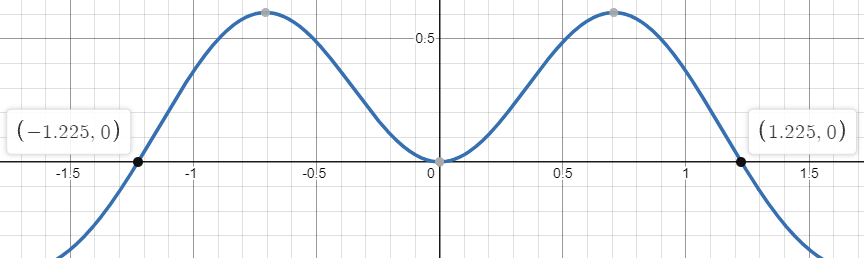
\includegraphics[scale=0.5]{exercise_1_solution_graph.png}
	\vfill
	\small
	Because $g'(x)$ changes signs at $x=-1.225\text{, }1.225$, local extrema are $g(-1.225)$ and $g(1.225)$.
	\[g(-1.225)=-0.410\text{; }g(1.225)=0.410\]
	\[\boxed{\text{Local Maximum: }0.410\text{; Local Minimum: }-0.410}\]
\end{frame}
\end{document}